\subsectionold{Запись за пределы массива}

Итак, мы прочитали какое-то число из стека явно \IT{нелегально}, а что если мы запишем?

Вот что мы пишем:

\lstinputlisting{patterns/13_arrays/2_BO/w.c}

\subsubsectionold{MSVC}

И вот что имеем на ассемблере:

\lstinputlisting[caption=\NonOptimizing MSVC 2008]{patterns/13_arrays/2_BO/w_RU.asm}

Запускаете скомпилированную программу, и она падает. Немудрено. Но давайте теперь узнаем, где именно.

\clearpage
\myindex{\olly}

Загружаем в \olly, трассируем пока запишутся все 30 элементов:

\begin{figure}[H]
\centering
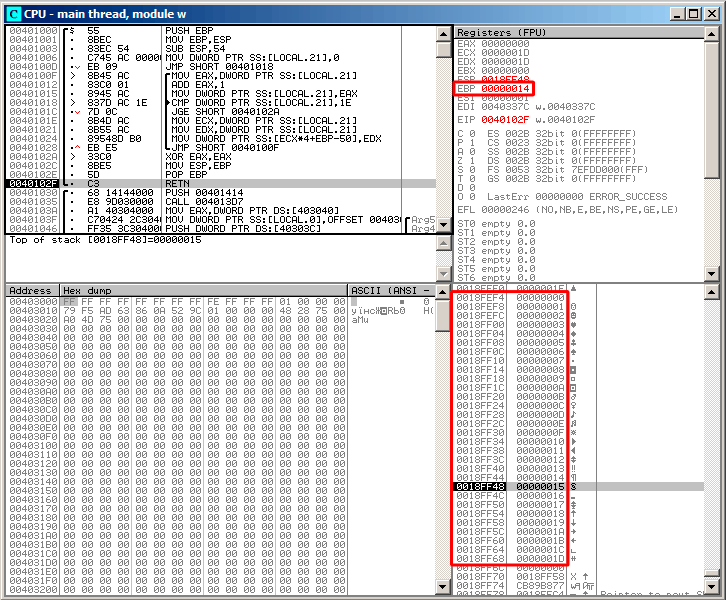
\includegraphics[scale=\FigScale]{patterns/13_arrays/2_BO/olly_w1.png}
\caption{\olly: после восстановления EBP}
\label{fig:array_BO_olly_w1}
\end{figure}

\clearpage
Доходим до конца функции:

\begin{figure}[H]
\centering
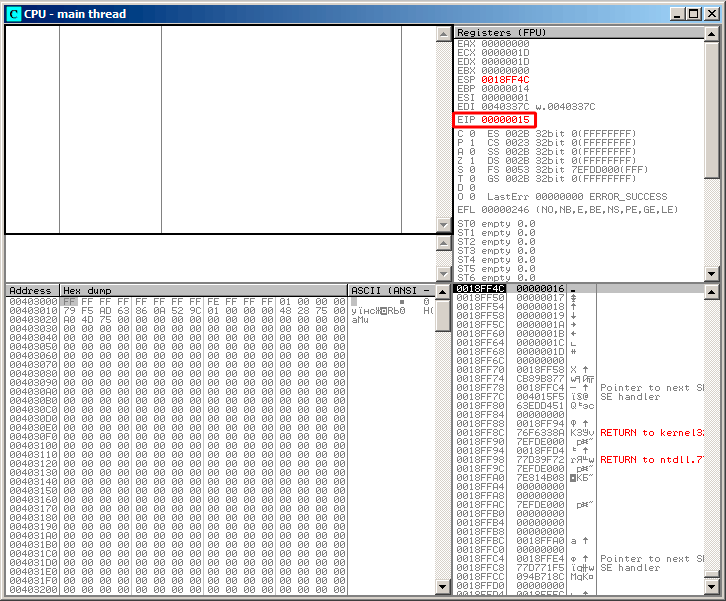
\includegraphics[scale=\FigScale]{patterns/13_arrays/2_BO/olly_w2.png}
\caption{\olly: EIP восстановлен, но \olly не может дизассемблировать по адресу 0x15}
\label{fig:array_BO_olly_w2}
\end{figure}

Итак, следите внимательно за регистрами.

\EIP теперь 0x15. Это явно нелегальный адрес для кода~--- по крайней мере, win32-кода! 
Мы там как-то очутились, причем, сами того не хотели. Интересен также тот факт, что в \EBP хранится 0x14, 
а в \ECX и \EDX хранится 0x1D.

Ещё немного изучим разметку стека.

После того как управление передалось в \main, в стек было сохранено значение \EBP. 
Затем для массива и переменной $i$ было выделено 84 байта. Это \TT{(20+1)*sizeof(int)}. 
\ESP сейчас указывает на переменную \TT{\_i} в локальном стеке и при исполнении следующего \INS{PUSH что-либо}, 
\IT{что-либо} появится рядом с \TT{\_i}.

Вот так выглядит разметка стека пока управление находится внутри \main:

\begin{center}
\begin{tabular}{ | l | l | }
\hline
  \TT{ESP}    & 4 байта выделенных для переменной $i$ \\
\hline
  \TT{ESP+4}  & 80 байт выделенных для массива \TT{a[20]} \\
\hline
  \TT{ESP+84} & сохраненное значение \EBP \\
\hline
  \TT{ESP+88} & адрес возврата \\
\hline
\end{tabular}
\end{center}

Выражение \TT{a[19]=что\_нибудь} записывает последний \Tint в пределах массива (пока что в пределах!).

Выражение \TT{a[20]=что\_нибудь} записывает \IT{что\_нибудь} на место где сохранено значение \EBP.

Обратите внимание на состояние регистров на момент падения процесса. В нашем случае 
в 20-й элемент записалось значение 20. 
И вот всё дело в том, что заканчиваясь, эпилог функции восстанавливал значение \EBP 
(20 в десятичной системе это как раз \TT{0x14} в шестнадцатеричной). 
Далее выполнилась инструкция \RET, которая на самом деле эквивалентна \TT{POP EIP}.

Инструкция \RET вытащила из стека адрес возврата (это адрес где-то внутри \ac{CRT}), которая вызвала \main),
а там было записано 21 в десятичной системе, то есть 0x15 в шестнадцатеричной. 
И вот процессор оказался по адресу 0x15, но исполняемого кода там нет, так что случилось исключение.

\myindex{\BufferOverflow}
Добро пожаловать! Это называется \IT{buffer overflow}\footnote{\href{http://go.yurichev.com/17132}{wikipedia}}.

Замените массив \Tint на строку (массив \Tchar), нарочно создайте слишком длинную строку, 
передайте её в ту программу, 
в ту функцию, которая не проверяя длину строки скопирует её в слишком короткий буфер, 
и вы сможете указать программе, по какому именно адресу перейти. 
Не всё так просто в реальности, конечно, но началось всё с этого.
Классическая статья об этом: \AlephOne.

\subsubsectionold{GCC}

Попробуем то же самое в GCC 4.4.1. У нас выходит такое:

\lstinputlisting{patterns/13_arrays/2_BO/w_gcc.asm}

Запуск этого в Linux выдаст: \TT{Segmentation fault}.

\myindex{GDB}
Если запустить полученное в отладчике GDB, получим:

\begin{lstlisting}
(gdb) r
Starting program: /home/dennis/RE/1 

Program received signal SIGSEGV, Segmentation fault.
0x00000016 in ?? ()
(gdb) info registers
eax            0x0	0
ecx            0xd2f96388	-755407992
edx            0x1d	29
ebx            0x26eff4	2551796
esp            0xbffff4b0	0xbffff4b0
ebp            0x15	0x15
esi            0x0	0
edi            0x0	0
eip            0x16	0x16
eflags         0x10202	[ IF RF ]
cs             0x73	115
ss             0x7b	123
ds             0x7b	123
es             0x7b	123
fs             0x0	0
gs             0x33	51
(gdb) 
\end{lstlisting}

Значения регистров немного другие, чем в примере win32, потому что разметка стека чуть другая.

